\section{geclusterte Instanzen wieder in Verse verwandeln} \label{Text2ClusterFile}
Um aus den geclusterten Instanzen wieder Verse zu machen, die in die jeweils passendes Cluster-Datei geschrieben werden, wird ein Programm namens Text2\-Cluster\-File entwickelt. Das Programm gruppiert anhand der Clusternummer und der Zeilennummer die Verse. So wird erkenntlich, welche Verse wie geclustert wurden. In Abbildung \ref{fig:AnalyseklassendiagrammText2ClusterFile} auf Seite \pageref{fig:AnalyseklassendiagrammText2ClusterFile} ist das Analyseklassendiagramm von Text2\-Cluster\-File zu sehen.

In Abbildung \ref{fig:AnalyseklassendiagrammText2ClusterFile} auf Seite \pageref{fig:AnalyseklassendiagrammText2ClusterFile} ist das Entwurfsklassendiagramm von Text2ClusterFile zu sehen.

\begin{figure}[htp]
\centering
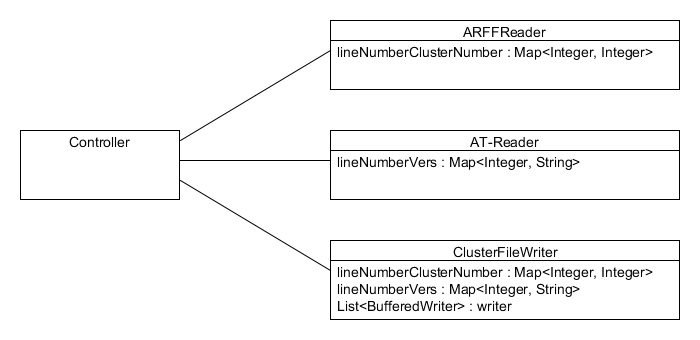
\includegraphics[width=1\textwidth]{Ingo/Bilder/AnalyseklassendiagrammText2ClusterFile.png}
\caption{Analyseklassendiagramm Text2ClusterFile}
\label{fig:AnalyseklassendiagrammText2ClusterFile}
\end{figure}

\begin{figure}[htp]
\centering
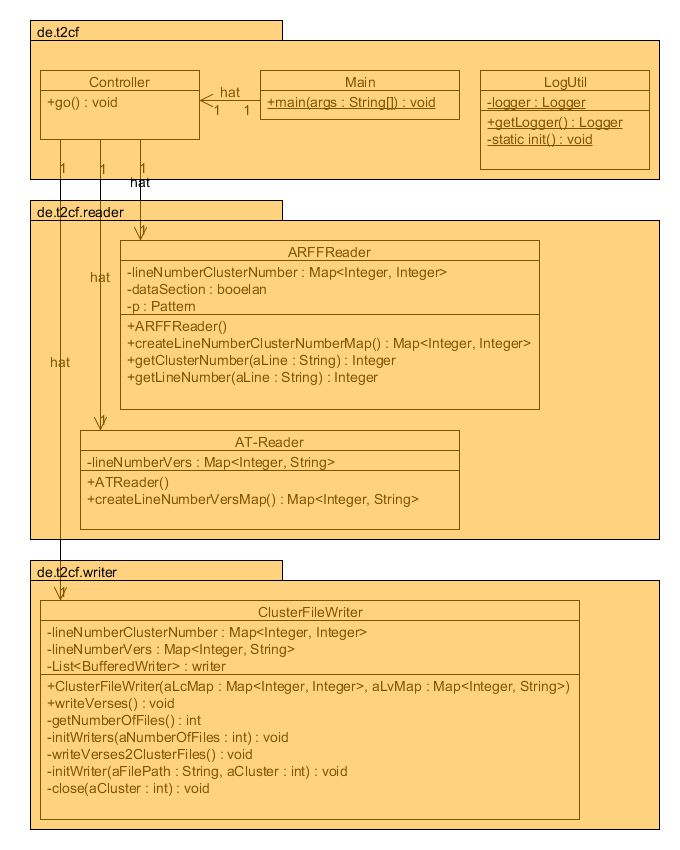
\includegraphics[width=1\textwidth]{Ingo/Bilder/EntwurfsklassendiagrammText2ClusterFile.png}
\caption{Entwurfsklassendiagramm Text2ClusterFile}
\label{fig:EntwurfsklassendiagrammText2ClusterFile}
\end{figure}